\documentclass[usenames,dvipsnames,aspectratio=169]{beamer}

\usepackage[utf8]{inputenc}
\usepackage[T1]{fontenc}
\usepackage[magyar]{babel}
\usepackage{indentfirst}
\usepackage{graphicx}
\usepackage{listingsutf8}
\usepackage{textcomp}
\usepackage{eurosym}
\usepackage{mathtools}
\lstset{literate=
  {á}{{\'a}}1 {é}{{\'e}}1 {í}{{\'i}}1 {ó}{{\'o}}1 {ú}{{\'u}}1
  {Á}{{\'A}}1 {É}{{\'E}}1 {Í}{{\'I}}1 {Ó}{{\'O}}1 {Ú}{{\'U}}1
  {à}{{\`a}}1 {è}{{\`e}}1 {ì}{{\`i}}1 {ò}{{\`o}}1 {ù}{{\`u}}1
  {À}{{\`A}}1 {È}{{\'E}}1 {Ì}{{\`I}}1 {Ò}{{\`O}}1 {Ù}{{\`U}}1
  {ä}{{\"a}}1 {ë}{{\"e}}1 {ï}{{\"i}}1 {ö}{{\"o}}1 {ü}{{\"u}}1
  {Ä}{{\"A}}1 {Ë}{{\"E}}1 {Ï}{{\"I}}1 {Ö}{{\"O}}1 {Ü}{{\"U}}1
  {â}{{\^a}}1 {ê}{{\^e}}1 {î}{{\^i}}1 {ô}{{\^o}}1 {û}{{\^u}}1
  {Â}{{\^A}}1 {Ê}{{\^E}}1 {Î}{{\^I}}1 {Ô}{{\^O}}1 {Û}{{\^U}}1
  {œ}{{\oe}}1 {Œ}{{\OE}}1 {æ}{{\ae}}1 {Æ}{{\AE}}1 {ß}{{\ss}}1
  {ç}{{\c c}}1 {Ç}{{\c C}}1 {ø}{{\o}}1 {å}{{\r a}}1 {Å}{{\r A}}1
  {€}{{\EUR}}1 {£}{{\pounds}}1 {ő}{{\H{o}}}1 {ű}{{\H{u}}}1
}
\lstdefinestyle{HTML}{
  language=HTML,
  breaklines=true,
  postbreak=\mbox{\textcolor{red}{$\hookrightarrow$}\space},
  stringstyle=\ttfamily,
  inputencoding=utf8,
  morekeywords={header, time, nav, main, article, section, aside, role, 
    footer, details, open, summary, srcdoc, list, datalist, placeholder, 
    pattern, required, min, max, step, enctype, formaction, formmethod, 
    formnovalidate, formtarget, output}
}
\usepackage{hyperref}
\usepackage{attachfile}
\usepackage{multirow}
% Navigációs pöttyök hozzáadása subsection nélküli fejezetekhez
\usepackage{remreset}
\makeatletter
\@removefromreset{subsection}{section}
\makeatother
\setcounter{subsection}{1}
%%%%%
\attachfilesetup{color={1.0 0.6 0.0},author={HFM},description={Kattintson duplán a minta %
megtekintéséhez!},icon=Paperclip}
\definecolor{kiemelesszin}{rgb}{0.6,0.0,0.0}
\definecolor{kiemelesszinZ}{rgb}{0.0,0.6,0.0}
\definecolor{kiemelesszinN}{RGB}{196,127,0}
\definecolor{hivatkozasszin}{rgb}{0.0,0.0,0.75}
\newcommand{\kiemel}[1]{{\color{kiemelesszin}#1}}
\newcommand{\kiemelZ}[1]{{\color{kiemelesszinZ}#1}}
\newcommand{\kiemelN}[1]{{\color{kiemelesszinN}#1}}
\newcommand{\hiv}[1]{{\color{hivatkozasszin}#1}}
\frenchspacing
\usetheme[compress]{Berlin}

\title[Web technológiák - HTML]{Web-technológia}
\subtitle{Cascading Style Sheets}
\author{Dr. Hatwágner F. Miklós}
\institute{Széchenyi István Egyetem, Győr}
\date{\hiv{\href{https://github.com/wajzy/GKxB\_INTM049.git}{https://github.com/wajzy/GKxB\_INTM049.git}}\\ \today}

\begin{document}

%1
\begin{frame}[plain]
  \titlepage
\end{frame}

\section{Alapok}

\subsection{Előnyök}

%2
\begin{frame}
  CSS: Cascading Style Sheets
  \begin{itemize}
    \item $\approx$ lépcsőzetes/sorba kapcsolt stíluslapok
    \item \emph{formázás, megjelenés} leírásának elválasztása a \emph{tartalomtól} (HTML), előnyei:
    \begin{itemize}
      \item külön fájlban tárolható, ami több weboldalhoz is használható, így csökken az összesített kódméret, 
      \item egységessé válik ezen oldalak megjelenése,
      \item egymástól függetlenül, egyidejűleg lehet szerkeszteni a formát és a tartalmat,
      \item gyorsabban módosítható a megjelenés, mert csak egy helyen kell változtatni,
      \item hatékonyabbá válik a gyorstárazás,
    \end{itemize}
    \item különféle médiára eltérő formázás lehetséges (pl. képernyő, nyomtatás)
    \item \hiv{\href{http://www.csszengarden.com/}{a CSS ereje}}
    \item \hiv{\href{https://www.w3.org/Style/CSS/learning.en.html}{hivatalos W3C oldal}}
  \end{itemize}
\end{frame}

\subsection{Formázás HTML elemekkel és CSS-sel}

%3
\begin{frame}
  \small
  \begin{alertblock}{Elavult módszer (\textattachfile{htmlFormazas.html}{htmlFormazas.html})}
    \lstinputlisting[style=HTML,numbers=left]{htmlFormazas.html}
  \end{alertblock}
\end{frame}

%4
\begin{frame}
  \scriptsize
  \begin{exampleblock}{Formázás CSS-sel (\textattachfile{cssFormazas.html}{cssFormazas.html})}
    \lstinputlisting[style=HTML,linerange={3-10},numbers=left,firstnumber=3]{cssFormazas.html}
  \end{exampleblock}
  \begin{exampleblock}{Formázás CSS-sel (\textattachfile{cssFormazas.css}{cssFormazas.css})}
    \lstinputlisting[style=HTML,numbers=left]{cssFormazas.css}
  \end{exampleblock}
\end{frame}

\subsection{Szintaktika}

%5
\begin{frame}[fragile]
  \begin{columns}[c]
    \column{0.5\textwidth}
      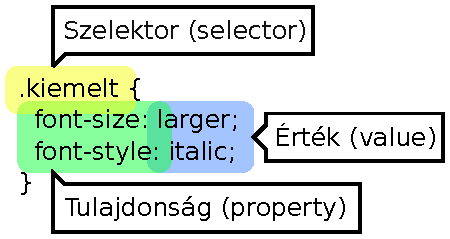
\includegraphics[scale=0.75]{szintakszis.pdf}\\
      \begin{block}{Deklaráció sablonja}
      \vspace{-0.5cm}
\begin{verbatim}
szelektor {
  tulajdonság1: érték(ek);
  tulajdonság2: érték(ek);
  ...
  tulajdonságN: érték(ek);
}
\end{verbatim}
      \vspace{-0.4cm}
      \end{block}
    \column{0.5\textwidth}
      \begin{description}[m]
        \item[Szelektor] \hfill \\ Mit akarunk formázni?
        \item[Tulajdonság] \hfill \\ Milyen tulajdonságán változtassunk?
        \item[Érték] \hfill \\ Milyen legyen az új állapot?
      \end{description}
  \end{columns}
  
\end{frame}

%6
\begin{frame}
  Megjegyzések a CSS-ben:
  \begin{itemize}
    \item \texttt{/* megjegyzes */}
    \item végleges kódból célszerű elhagyni
    \item Lehet több soros is
  \end{itemize} 
  \hiv{\href{https://jigsaw.w3.org/css-validator/}{CSS ellenőrző}}
\end{frame}

\subsection{Egyszerű szelektorok}

%7
\begin{frame}
  \begin{description}[m]
    \item[HTML elem neve] \hfill \\ \texttt{p \{ font-style: italic; \}}
    \item[Egyedi azonosító (\texttt{id} attribútum) alapján] \hfill \\ 
      \texttt{\#lablec \{ font-size: 10pt; \}}\\
      Az \texttt{id} nem kezdődhet számjegy karakterrel!
    \item[Univerzális szelektor, mindenre illeszkedik] \hfill \\ \texttt{* \{ font-size: smaller; \}}
  \end{description}
\end{frame}

%8
\begin{frame}
  \begin{description}[m]
    \item[Osztály (\texttt{class} attribútum alapján)] \hfill \\ 
      \texttt{*.kisbetus \{ font-size: small; \} /* bármilyen HTML elemhez */} \\
      \texttt{.kisbetus \{ font-size: small; \} /* bármilyen HTML elemhez, rövid alak */}\\
      \texttt{p.voros \{ color: red; \} /* csak adott (pl. <p>) HTML elemhez */}\\
      A \texttt{class} értéke nem kezdődhet számjeggyel, de lehet egyszerre több, szóközzel elválasztott értéke: \\
      \texttt{<p class="kisbetus voros">Apróbetűs piros bekezdés</p>}
    \item[Elemek csoportosítása] \hfill \\ \texttt{h1, h2, h3 \{ font-family: Arial; \}}
  \end{description}
\end{frame}

%9
\begin{frame}
  \begin{exampleblock}{\textattachfile{egyszeruSzelektor.html}{egyszeruSzelektor.html}}
    \scriptsize
    \lstinputlisting[style=HTML,linerange={3-13},numbers=left,firstnumber=3]{egyszeruSzelektor.html}
  \end{exampleblock}
\end{frame}

%10
\begin{frame}
  \begin{exampleblock}{\textattachfile{egyszeruSzelektor.html}{egyszeruSzelektor.html}}
    \scriptsize
    \lstinputlisting[style=HTML,linerange={14-15},numbers=left,firstnumber=14]{egyszeruSzelektor.html}
  \end{exampleblock}
\end{frame}

%11
\begin{frame}
  \begin{exampleblock}{\textattachfile{egyszeruSzelektor.css}{egyszeruSzelektor.css}}
    \scriptsize
    \lstinputlisting[style=HTML,numbers=left]{egyszeruSzelektor.css}
  \end{exampleblock}
  \begin{center}
    
\includegraphics[width=.9\textwidth]{egyszeruSzelektor.png}
  \end{center}
\end{frame}


\end{document}
